%% fig07-batch-mu-axis, caption is in docs/figures/README.md
\documentclass[border=8pt]{standalone}
% Shared preamble for the interpolation-geometry figures.
% \input by every figNN-*.tex. 
\usepackage[T1]{fontenc}
\usepackage{amsmath,amssymb}
\usepackage{tikz}
\usetikzlibrary{shapes.misc,arrows.meta,calc,decorations.pathreplacing,positioning,fit,backgrounds}

\definecolor{ink}{HTML}{1A1A1A}
\definecolor{gridc}{HTML}{9AA3AD}
\definecolor{accent}{HTML}{1F5FA9}
\definecolor{good}{HTML}{2E7D4F}
\definecolor{bad}{HTML}{B03030}
\definecolor{soft}{HTML}{E6EDF7}
\definecolor{softg}{HTML}{E3F0E8}
\definecolor{softr}{HTML}{F8E6E6}
\definecolor{amber}{HTML}{B8860B}


\tikzset{
  gpt/.style={circle,fill=ink,inner sep=1.15pt},
  ghost/.style={circle,draw=gridc,fill=white,inner sep=1.15pt},
  dep/.style={cross out,draw=accent,thick,inner sep=1.6pt,minimum size=4pt},
  traj/.style={gridc,dotted,thick,-{Stealth[length=2mm]}},
  htraj/.style={accent,very thick,-{Stealth[length=2.6mm]}},
  lbl/.style={font=\footnotesize},
  slbl/.style={font=\scriptsize},
}

\begin{document}
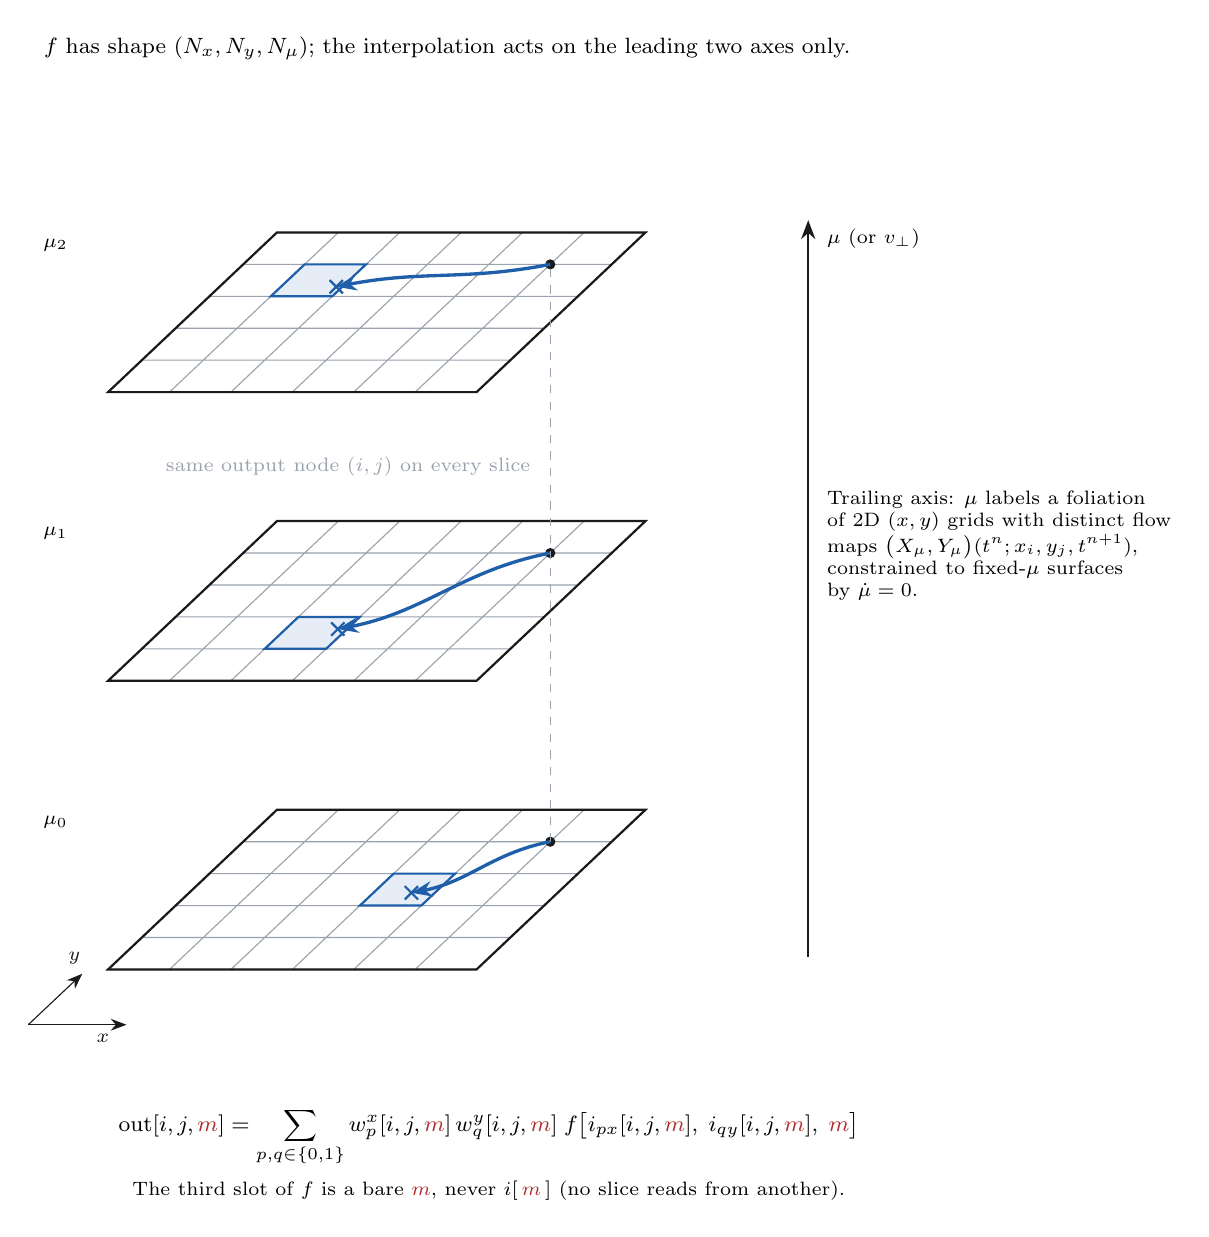
\begin{tikzpicture}[x=0.78cm,y=0.78cm]
  \newcommand{\muslice}[7]{%
    \begin{scope}[shift={(#1,#2)}]
      \begin{scope}[cm={1,0,0.55,0.52,(0,0)}]
        \fill[white,opacity=0.94] (0,0) rectangle (6,5);
        \draw[gridc,thin] (0,0) grid[step=1] (6,5);
        \draw[ink,thick] (0,0) rectangle (6,5);
        \fill[soft,opacity=0.95] (#6) rectangle ++(1,1);
        \draw[accent,thick] (#6) rectangle ++(1,1);
        \node[circle,fill=ink,inner sep=1.3pt] at (5,4) {};
        \coordinate (#7) at (5,4);
        \draw[htraj] (5,4) to[out=205,in=25] (#4,#5);
        \node[dep] at (#4,#5) {};
      \end{scope}
      \node[slbl,anchor=east] at (-0.5,2.4) {#3};
    \end{scope}}
  \muslice{0}{9.4}{$\mu_2$}{1.90}{3.30}{1,3}{arrB}
  \muslice{0}{4.7}{$\mu_1$}{2.85}{1.62}{2,1}{arrM}
  \muslice{0}{0}{$\mu_0$}{3.62}{2.40}{3,2}{arrA}
  \draw[gridc,dashed] (arrA) -- (arrM) -- (arrB);
  \node[slbl,gridc,anchor=east,fill=white,inner sep=1.5pt] at ($(arrM)+(-0.25,1.4)$) {same output node $(i,j)$ on every slice};
  % axes on the bottom slice
  \draw[-{Stealth[length=2mm]},ink] (-1.3,-0.9) -- (0.3,-0.9) node[slbl,anchor=north,xshift=-0.3cm] {$x$};
  \draw[-{Stealth[length=2mm]},ink] (-1.3,-0.9) -- ($(-1.3,-0.9)+(0.88,0.83)$) node[slbl,anchor=south east,xshift=0.1cm] {$y$};
  \draw[-{Stealth[length=2.4mm]},ink,thick] (11.4,0.2) -- (11.4,12.2);
  \node[slbl,anchor=west] at (11.55,11.9) {$\mu$ (or $v_\perp$)};
  \node[slbl,anchor=west,align=left] at (11.55,6.9)
     {Trailing axis: $\mu$ labels a foliation\\
      of 2D $(x,y)$ grids with distinct flow\\
      maps $\big(X_\mu,Y_\mu\big)(t^{n};x_i,y_j,t^{n+1})$,\\
      constrained to fixed-$\mu$ surfaces\\
      by $\dot\mu=0$.};
  \node[lbl,anchor=west,align=left] at (-1.2,15.0)
     {$f$ has shape $(N_x,N_y,N_\mu)$; the interpolation acts on the leading two axes only.};
  \node[anchor=north,align=center] at (6.2,-2.1)
  {\footnotesize
   $\displaystyle \mathrm{out}[i,j,{\color{bad}m}]=\sum_{p,q\in\{0,1\}}
     w^x_p[i,j,{\color{bad}m}]\,w^y_q[i,j,{\color{bad}m}]\;
     f\big[i_{px}[i,j,{\color{bad}m}],\;i_{qy}[i,j,{\color{bad}m}],\;{\color{bad}m}\big]$\\[4pt]
   \scriptsize The third slot of $f$ is a bare ${\color{bad}m}$, never
   $i[\,{\color{bad}m}\,]$ (no slice reads from another).};
\end{tikzpicture}
\end{document}
